\section{Résultats des métriques}
  L'intervalle entre chaque batch a été fixé à 1 seconde. Ainsi, Spark va récupérer pendant 1 seconde les tweets grâce à l'API de Twitter, effectuer les opérations de statistiques sur ces tweets et restituer l'information, dans notre cas, sous forme d'affichage à l'écran.

  \subsection{Time behaviour}
    Une des catégories de métriques est la notion de temps. En effet, pour l'analyse en temps réel, il est nécessaire de connaître les durées de chaque action afin de déterminer d'éventuel goulot d'étranglement. Pour notre prototype, nous avons mis en place une métrique sur la durée pour effectuer un batch complet, à savoir la récupération des tweets et le calcul de statistiques sur celui-ci. Une deuxième métrique a été mise en place dans le but de relever la durée nécessaire seulement pour réaliser les statistiques sur les tweets d'un batch. La figure~\ref{fig:resultats_stat_tweet} présente les résultats obtenus. \\

    \begin{figure}
      \centering
      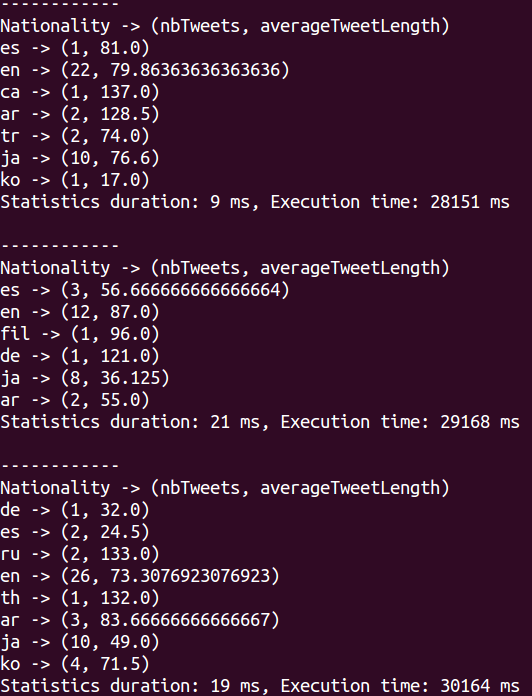
\includegraphics[width=0.6\textwidth]{images/stat_results.png}
      \caption{Résultats de l'analyse de tweet en temps réel}
      \label{fig:resultats_stat_tweet}
    \end{figure}

    Nous pouvons observer trois batch différents. Cela correspond donc à un temps d'exécution théorique de streaming de trois secondes (car nous avions spécifié un intervalle de 1 seconde comme paramètre). Cela est confirmer d'un point de vue exécution grâce à la métrique \emph{Execution time} présent sur la figure~\ref{fig:resultats_stat_tweet}. Nous pouvons remarquer que cette métrique prend respectivement les valeurs 28151, 29168 et 30164 millisecondes. Il y a donc bien 1 seconde entre chaque retour de résultats. \\

    La deuxième métrique est nommée \emph{Statistics duration} est prend respectivement les valeurs 9, 21 et 19 millisecondes. Le temps de calcul des statistiques sur les tweets d'un batch est bien inférieur au temps entre chaque batch et donc le calcul de ces statistiques n'est pas un goulot d'étranglement.

  \subsection{Resources utilization}

  \subsection{Installability}

\section{Sources pour l'implémentation du prototype}
  \url{https://spark.apache.org/docs/latest/streaming-programming-guide.html}
